%%%%%%%%%%%%%%%%%%%%%%%%%%%%%%%%%%%%%%%%%%%%%%%%%%%%%%%%%%%%%%%%%%%%%%%%%%%%%%%%
% experiment.tex: Chapter describing the experiment
%%%%%%%%%%%%%%%%%%%%%%%%%%%%%%%%%%%%%%%%%%%%%%%%%%%%%%%%%%%%%%%%%%%%%%%%%%%%%%%%
\chapter{Hadron Collider and Detector}
This section describes the particle accelerator and detectors that are used to produced and detect particles at colliders. The first section describes the particle accelerator while the following section describes the CMS detectors with emphasis to those sections which are directly relevant to this analysis. A detailed description of the LHC and detectors can be found in \cite{LHC} and \cite{CMSD}.
\section{Large Hadron Collider}
\subsection{Overview}
The Large Hadron collider~(LHC) is a proton-proton and heavy ion collider designed to achieve a center of mass $\displaystyle{\sqrt{S}}$ energy of 14~TeV. It is hosted and controlled by the European Organisation for Nuclear Research~(CERN). Unlike linear colliders, the LHC is a circular collider with nearly 27~km in circumference located at the border between France and Switzerland. It is designed to smash protons and ions against each other controlled by powerful magnets at officially four main locations. At each major collision point are multi-purpose particle detectors ranging from A Toroidal LHC Apparatus~(ATLAS) and Compact Muon Solenoid~(CMS) both non-fixed target detectors, A Large Ion Collider Experiment~(ALICE) for colliding heavy ions and finally Large Hadron Collider beauty~(LHCb), a fixed target experiment for investigating the properties of B-Hadrons. We  give a full description of the important parts of the LHC in the following subsections, detail discussion of other interesting parts can be found here \cite{LHC}.
There are three main steps prior to colliding protons or ions at the LHC.  The first is ramping up the energy of the beams followed by squeezing the beams at interaction points( CMS or ATLAS) and finally remove the separator bumps that are formed by local corrector magnets.
Thus our description of the LHC will follow this three stages.
\begin{center}
\centering
\mbox{
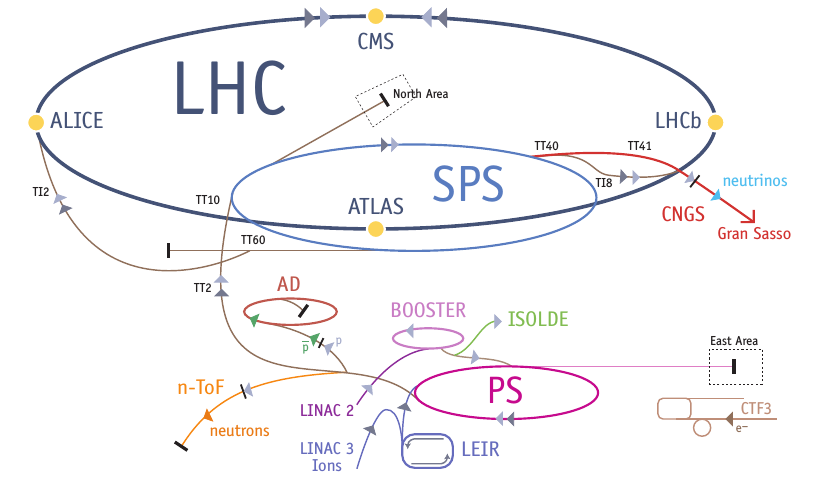
\includegraphics[width=6in]{THESISPLOTS/The_LHC.png}}
\captionof{figure}{Schematic diagram showing the full Large hadron Collider. Image taken from \cite{LHCB}}
\label{fig:LHC}
\end{center}
\subsection{Colliding Energy}
Hydrogen gas is inserted into a linear accelerator called Linac2 where they are stripped off of their orbiting electrons to become hydrogen ions or protons. Under the influence of electric fields, these protons are accelerated to an energy of 50~\MeV creating a stream of particles called \textit{particle beams}. These beams are arranged in packets known as \textit{bunches}. Particle acceleration if provided through the use of Radio-Frequency~(RF) cavities containing electromagnetic fields which oscillate at a particular frequency. The protons surf this electromagnetic fields and are group in troughs of the electromagnetic waves called RF~\textit{buckets}. The circular nature of the synchrotron accelerator ensures that the protons pass many times through a cavity and during each time their energy can be slowly increase to reach the design energy.
The 50~\MeV protons from the Linac2 are injected into the proton synchrotron Booster~(PSB). The PSB accelerates the protons to up to 1.4~\GeV and inject them into the Proton Synchrotron~(PS) which pushes the protons energy to 25~\GeV. These protons travelling at 99.93\% the speed of light are sent to the Super Proton Synchrotron~(SPS) and accelerated to an energy of 450~\GeV. They are finally transferred into the LHC ring(both in a clockwise and anti-clockwise direction) and accelerated for about 20 minutes to their norminal energy of 7~\TeV. As this point these protons are travelling with the speed of 99.9999\% the speed of light. Powerful magnets are used to keep the beeps travelling in the circular LHC ring. The advantage of circular particle colliders such as the LHC over fix target colliders is that, the energy available to make new particles called the center of mass energy denoted as $\sqrt{S}$ is simply the sum of the energy of the two beams i.e $\sqrt{S} = \mathit{E}_{\mbox{beam1}} +   \mathit{E}_{\mbox{beam2}}$ compared to $\sqrt{\mathit{E}_{\mbox{beam}}}$ for fix target experiments. In the case of the LHC, each beam is designed to have energy of 7~\TeV and that makes $\sqrt{S} = 14$~\TeV. Although in circular collider, an accelerating charge particles like the proton would loose energy in for the form of radiation which is inversely proportional to the mass of the charge particle to the fourth power requiring  the need for continuous addition of energy after each turn to maintain the beam energy to a stable value. Since the proton's mass is  about $0.938$~\GeV which is close to 1~\GeV, this lost of energy is not very significant unlike  electrons  whose mass of about $0.000511$~\GeV making their energy lose through radiation more and thus less preferable to use as the main particles for a circular hadron collider. However, the debris of particles produced when electrons collide is much less compared to that of hadrons making analysis in a hadron collider more challenging. 
\subsection{Luminosity}
Luminosity is the measurement of the number of collisions that can be produced in a collider per squared area per second. This is known as the instantaneous luminosity and it is related to the cross-section(a probabilistic measure of the possibility of a given collision process happening) through the equation:

\begin{equation}
N_{\mbox{events/sec}} = \mbox{Luminosity} \cdot \mbox{Cross Section}
\end{equation}
where the luminosity $\mathscr{L}$ is related to the total integrated luminosity(delivered luminosity over time) $\mathrm{L} = \int \mathscr{L}dt$ and is defined in terms of accelerator(assuming round beams and equal values of beta function) parameters as:
\begin{equation}\label{lumi}
\mathscr{L} = \frac{1}{4\pi}\cdot\left(f_{rev}\mathit{n}_{b}\mathit{N}_{b}\right)\cdot\frac{\mathit{N}_{b}}{\varepsilon_{N}}\cdot \frac{\gamma}{\beta^{\ast}}\cdot \mathscr{R}(\theta_{c},\varepsilon,\beta^{\ast},\sigma_{z} )
\end{equation}

where $\mathit{N}_{b}$ is the number of particles per bunch, $\mathit{n}_{b}$ is the number of bunches, $f_{rev}$ is the revolutionary frequency, $\gamma = E/m_{p}$ is the relativistic factor, $\varepsilon_{N}$ is the normalised beam emittance which along with $\beta^{\ast}$, the value of the amplitude or beta function at interaction point, determines the size of the beam. $\mathscr{R}$ is the geometrical reduction factor arising from the fact that the beams to not collide head-on but at a non-zero angle called the crossing angle or \textit{"Piwinski angle"}( $\phi \equiv \frac{\theta_{c}\sigma_{z}}{2\sigma_{x}}$). This effect is known as the \textit{hour-glass effect}.
From the above definition \eqref{lumi}, it is evident that keeping the emittance (meaning particles in beam are confined to a small distance and have nearly the same momentum ) means the likelihood of particle interaction will be greater and thus higher luminosity. However this is often not easy to archive as increasing the beam energy means reducing the beam emittance. The normalized emittance $\varepsilon_{N}$ is often used as its dependence on beam energy is a squared root dependence.
In the same way, lower beta values implies the width of beam is narrower or properly \textit{"squeezed"} at interaction point resulting to an increase in number of collisions hence higher luminosity.
This squeezing of depends on the quadruple magnet configuration and powering. 
In addition to low beam emittance and lowest value of beta function at interaction point($\beta^{\ast}$), one can also archive higher luminosity by using high population bunches($\mathit{N}_{b}$) and collide them at high frequency.
\paragraph*{Luminosity Measurement}\mbox{}\\
Obviously using equation \eqref{lumi} to determine the instantaneous and integrated luminosity would involve a lot of uncertainty in the measurements of about 20-30\%, as there are so many parameters whose value need to be measured precisely in a normal LHC operation. Rather specialised LHC runs known as \textit{"Van der Meer Scans"}\cite{lhclumi} are used to calibrate specialized equipments used for determining luminosity.
%The method employed by CMS(using TOTEM) is to use the total proton-proton~(\textit{p-p} cross section. 
The method employed by CMS is using the Hadronic Foward~(HF) calorimeter to make luminosity measurements.
Using production rates or cross sections of well and precisely calculable processes and rewriting \eqref{lumi} as:
\begin{equation}
 \mathscr{L} \equiv \frac{Rate_{tot}}{\sigma_{tot}}    = \frac{\mu \mathit{n}_{b} f_{rev}}{\sigma_{tot}} 
\end{equation}
where $\mu = \left\langle \mathit{N}_{tot}/ \mathit{n}_{b} \right\rangle $ is the \textit{average number of interactions per bunch crossing}.
CMS keeps track of "recorded" and "delivered" luminosity. Delivered luminosity refers to the luminosity delivered by LHC to CMS and one would expect this to be equal to  the amount recorded. However, there are instances where the CMS detector is unable to take data either because the data acquisition chain~(DAC) is busy or one of the CMS sub-detectors is temporarily down. Part of my job as a sub-detector expert during CMS data taking of LHC Run 1 was to make sure that the period of temporal unavailability of the ECAL sub-detector is as minimal as possible.
\begin{center}
\centering
\mbox{
%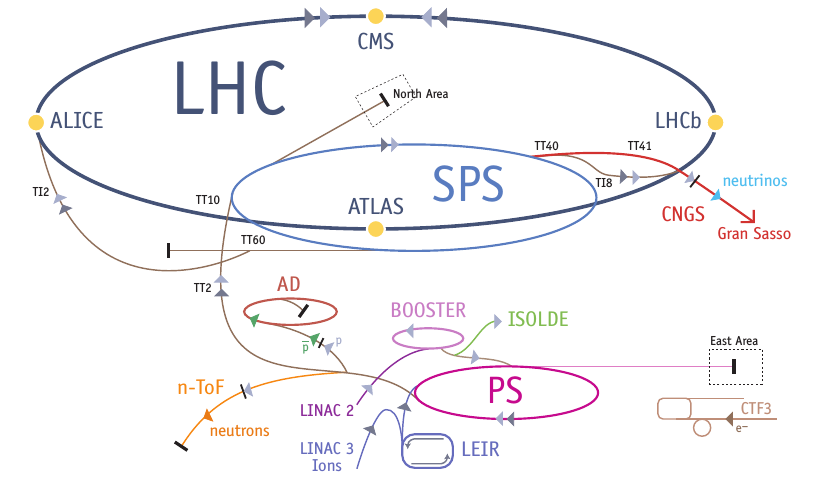
\includegraphics[width=6in]{THESISPLOTS/The_LHC.png}
}
\captionof{figure}{Recorded luminosity by CMS detector and LHC delivered luminosity in days/months during LHC Run 1 2012 operation.}
\label{fig:cmslumi}
\end{center}

  
%of well understood and calculable processes such as the production of $\mathrm{W}$ and $\mathrm{Z}$ bosons or di-leptons via  two photon exchange. 
\subsection{Superconducting Electromagnets}
The LHC design and operation uses a total of 9593 powerful magnets of different types for different purposes. Since there are two beams of protons running in clock-wise and anti-clock wise directions, the LHC uses an ingenious technique design  of the magnetic field in every dipole magnet generates a vector field $\mathbb{B}$ in each pipe pointing in opposite direction to that of the other but both always perpendicular to the beam directions. The Lorentz or magnetic force acting on the protons in both pipes always point towards the center thus keeping the beams in circular motion. In circular accelerators as the LHC and its smaller synchrotron rings, given the accelerator radius,$R$, the beam energy $p$ is determined by the strength $\mathbf{B}$ of the magnetic field. This can be easily understood using the Lorentz force  such that $\displaystyle{p[TeV] = 0.3\mathbf{B}[T]\cdot R[km] }$.
The LHC is is a 26.659~km in circumference machine using powerful dipole magnets with magnetic field strength of about 8.33~Tesla(T) are 7~TeV to keep the protons circulating in their curved path or orbits. The LHC operates using superfluid helium for heat transport at 1.4~K(-271.3~$^{\circ}C$)  temperature to prevent these near 1232 dipole magnets, 858 quadruple and 6208 correcting magnets from overheating due to the energy stored in these magnets. Conventional magnetics aren't convenient for modern particle accelerators with high center of mass energy for both performance and economic reason. Rather, superconducting magnets made with modern technology using  niobium-tantanium~(Nb-Ti) filaments strands or cables are used to provide the high magnetic field required. 
%These magnetics provide a magnetic field strength of about 8.33~T and are kept at about 1.4K in temperature during LHC operation.

Quadrupole electromagnet and correcting magnets are  used to keep the particles in the beam and archive the required focus and de-focusing needed. At interaction point, the quadrupole magnets are held symmetrically around the beam pipe to help squeeze the proton beams to very low values of beta function thus ensuring that many particle collisions as possible necessary for higher luminosity.


\subsection{Timing}
The Large Hadron Collider (LHC) is designed to collide proton-proton (pp) bunches every  24.95~ns at designed luminosity. This means, the distance between each proton bunch is about 7.5~m compared to the nearly 100~m of optical fibre length which is required to transport readout information from the very front end electronics on the detectors to the back end  electronics at Point 5 for processing.
It is therefore imperative to have a data synchronisation system for the trigger and readout systems of the LHC experiments in order that events from every proton-proton collision are properly assigned to the particular bunch crossing ~(BX) which produced them.
The LHC is equipped with a Timing, Trigger and Control~(TTC) system with a bunch clock frequency of 40.07897~MHz whose function is to distribute synchronized LHC time to all the detectors including CMS.
Timing synchronisation in the LHC is achieved using a Beam Synchronous Timing ~(BST) system which distributes timing using the LHC revolution frequency(at 11.246~kHz) or LHC orbit  and the RF bunch crossing frequency(40.07897~MHz at 7~\TeV). 
Thus, the LHC fast timing signals from the RF generators  of the machine and orbit signals are distributed from the Prevessin Control Room~(PCR) through single-mode optical fibers(about 10.1~km in length for CMS) to all LHC experiments,  test beam areas, beam instrumentation around the ring and the SPS transfer lines.  At CMS counting room, the LHC clock and orbit signals  are recovered in the TTC Machine Interface crate~(TTCmi) and later distributed to the Trigger Control and sub-detector master TTC crates. All Level1~(L1) trigger and Data Acquisition~(DAQ) pipelines are driven with a 24.95~ns cycle clock locked to the LHC machine clock. The phase difference between the LHC 40~MHz clock and the arrival of detector signals from collision to the front-end electronics must be determined and adjusted for and monitored. The determination and assignment of pulses to bunch crossings depends critically on this initial clock phase adjustments and stability. This amplitude or pattern(also known as trigger primitives) for each trigger and bunch crossing is transmitted to the regional trigger logic in digital form every crossing and is synchronised with the LHC clock. Each trigger primitive digital data is then assigned to clock cycle in a process known as bunch crossing assignment. a   Detail expert description of LHC unified timing distribution system can be found here \cite{LHCT, LHCT1, LHCT2, LHCT3}.
%This means that there is the possibility of producing a LL particle when two protons collide every 25~ns.
%Thus it becomes a serious challenge  for triggering, data acquisition and associating the correct emerging particle to
%the correct bunch crossing (BX).
 %This is even more challenging for LL particles produced with low velocity since
%by design and read-out, with the time separation of 25~ns between BXs,
%Particles produced from LHC are assumed to be travelling at the speed of light (c = 299 792 458~m$s^{-1}$).
%Thus, such light speed particles will travel a distance of $\approx 7.5$~m.
%This leads to the possibility of having about 3 BXs  simultaneously contained in the Compact Muon Solenoid~(CMS) detector.
%As a result, LL particles produced with slower velocity might cause triggers to assigned particles to the wrong BX and so reduced the trigger
%efficiency for LL particles. An interesting study has been done by the another multi-purpose detector at CERN, ATLAS
%which looked at LL particle with different velocities~ $\beta$ and showed that it is important to enlarge triggering windows so as to increase
%triggering efficiencies for low velocity particles.

\begin{center}
\begin{minipage}[b]{1.0\linewidth}
\centering
 %\setlength{\abovecaptionskip}{0pt}
  %\setlength{\belowcaptionskip}{10pt}
 % \topcaption{GMSB,GGM Phenomenology and Relevant final states}
  \begin{tabular}{|l|l|l|l|l|}
  \hline \hline
  \multicolumn{5}{|c|}{\bfseries{LHC Operation Parameters 2010-2013}} \\
  \hline \hline
  \bfseries{Parameter} & \bfseries{2010 value} & \bfseries{2011 Value} & \bfseries{2012/13 Value} & \bfseries{Design Value} \\
   \hline \hline
 Beam energy[Te] & 3.5  & 3.5  & 4.0  & 7 \\ 
  \hline
  $\beta^{\ast}$ in IP 5[m] & 3.5 & 1.0 & 0.6  & 0.55 \\
  \hline
  Bunch spacing [ns]& 150 & 75/50 & 50 & 25 \\
  \hline
  Number of bunches & 368 & 1380 & 1380 & 2808 \\
  \hline
  Protons/bunch  & $1.2 \times 10^{11}$ & $1.45 \times 10^{11}$ &  $1.7 \times 10^{11}$& $1.15 \times 10^{11}$ \\
  \hline
  Normalised emittance[mm.rad] & $\approx 2.0$ & $\approx 2.4$ & $\approx 2.5$ &  3.75\\
  \hline
  Peak luminosity[$cm^{-2}s^{-1}$]& $2.1 \times 10^{32}$ & $3.7 \times 10^{33}$ & $3.7 \times 10^{33}$ & $1 \times 10^{34}$ \\
  \hline
  Evts/bunch crossing & 4 & 17 & 37 &  19 \\
  \hline
  Stored Beam energy(MJ)& $\approx 28$ &  $\approx 110$  & $\approx 140$  & $\approx 362$ \\
  \hline
  Int. Luminosity by CMS[$pb^{-1}$]&  &  &  &  \_ \\
 \hline
 Circumference[km]  &26.659 & 26.659 & 26.659 & 26.659 \\
 \hline
 Dipole Magnet B[T] & 8.33 & 8.33 & 8.33 & 8.33 \\
 \hline  
  \end{tabular}
  \captionof{figure}{The LHC operation parameter conditions during RUN 1:2010-2013}
 \end{minipage}
 \end{center}


\subsubsection{LHC Bunch Structure}
An LHC orbit is made of about 3564 \textit{bunch} places. However only 2808 are occupied with protons. The bunch structure is archived by  breaking a continuous proton beam into pulsed beam of separate bunches using an electromagnetic field  with oscillating frequency of 400~MHz(LHC ring) in the SPS and LHC RF cavity. Thus each bunch is in an RF bucket. Each RF bucket has an energy against time profile as can be seen in figure below. The LHC filling scheme is arranged such that not all RF buckets have proton bunches. Thus there are empty buckets or beam gaps with missing bunches. These gaps are necessary to make  room for the rise/fall times at SPS/LHC injection and ejection and abort kickers magnets during say LHC beam dump. The time separation between two buckets/bunches filled or unfilled is about 2.5~ns. Filling and acceleration at each RF cavity point is performed so that there are about $10^{11}$protons/bunch. However, during filling and eventual bunch splitting at the PS, it is possible that some empty buckets are filled with a much smaller proton population compared to the main bunch. These less proton populated buckets can be $\Delta t$ = 2.5, 5.0, 7.5, $\ldots$~ns, trailing the main bunch labelled as Beam1 or Beam2 otherwise leading the main bunch with $\Delta t$ = -2.5, -5.0s, -7.5, $\ldots$~ns. If these less populated bunches are 2.5~ns spaced in time from each other, they are referred to as \textit{Ghost} bunches and if 5.0~ns, they are referred to as \textit{satellite} bunches see figure \eqref{fig:LDM-Ghost}.

\begin{center}
\centering
\mbox{
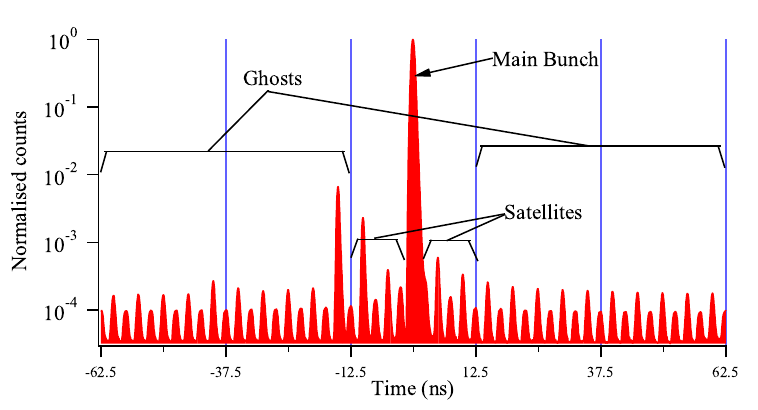
\includegraphics[width=4.5in]{/home/tensr/Dropbox/PHD_Thesis_HEP/PHD_THESIS/PHD/THESISPLOTS/Ghost-Satellite-Bunches-LDM.png}} 
\captionof{figure}{Longitudinal Profile taken with LDM detector showing definition of Ghost/Satellite bunches with respect to main bunches.}
\label{fig:LDM-Ghost}
\end{center}
The presence of ghost/satellite bunches increase the uncertainty in LHC luminosity measurements and can also generate proton-proton interactions in the collision region. Effects on ghost/satellite bunches on instantaneous luminosity measurements have been studied by both CMS, ATLAS and ALICE detectors \cite{ATLAST-GHOST} 
with their profile compared to main bunch bunches. CMS uses energy deposits in the endcap calorimeters with time space equivalent to those of ghost/satellite bunches while in ATLAS, they have also introduced a new detector called the Longitudinal Density Monitor~(LDM) to study ghost/satellite bunches. The results are shown in the figure \eqref{fig:CMS-ATLAS-Ghost}.
\begin{center}
\centering
\mbox{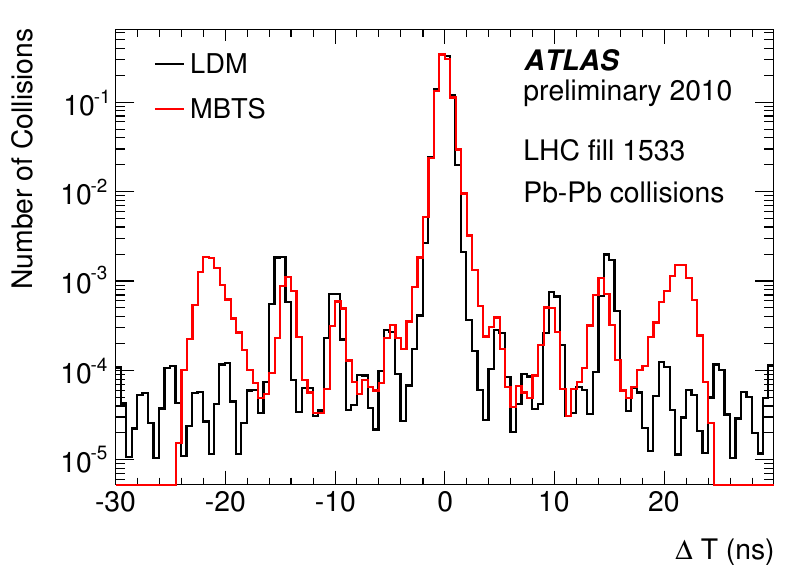
\includegraphics[height=2.5in,width=2.5in]{THESISPLOTS/ATLAS-LDM-GHOST.png} \quad \quad
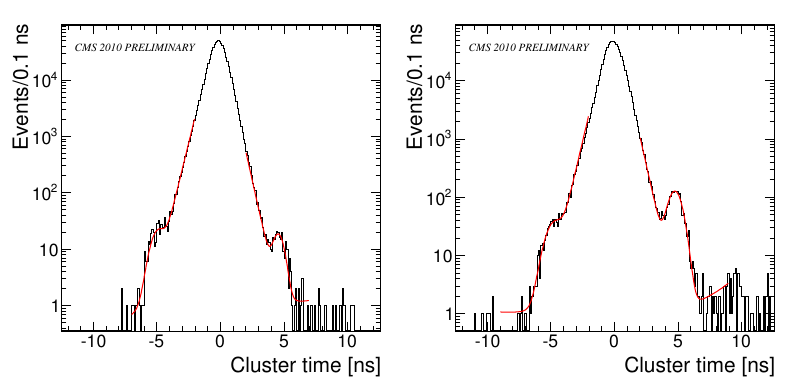
\includegraphics[height=2.5in,width=3.0in]{THESISPLOTS/CMS-Ghost-Profile.png}} 
\captionof{figure}{(left) Arrival time distribution(red) of ATLAS MBTS  for LHC fill 1533 during 2010 Pb-Pb run and LDM profile(black) for Beam2(same for Beam1).\newline
(Right) Timing of Clusters in the CMS endcap calorimeters for fill 1089:Left: EEP detector(left side of IP $z< 0$) Right: EEM detector( right side of IP, $z>0$). NB: Plots taken from \cite{ATLAS-GHOST} and \cite{CMS-GHOST}}
\label{fig:CMS-ATLAS-Ghost}
\end{center}
There is the possibility that ghost/satellite - ghost/satellite and ghost - Beam1/Beam2 collisions will happen generating events at the CMS detector. This is a major background in the search for delayed photons or objects in general as these collisions can occur \textit{in-time}(Beam1- Beam2) collisions or \textit{out-of-time} collisions. It is thus imperative to be able to quantify this contributions in any search analysis. We will show in future studies we have performs to both \textit{"guestimate"} and quantify these contributions in our search analysis.
\paragraph*{Beam Halo}\mbox{}\\
In addition to ghost/satellite bunches generating collisions events during collision, protons in ghost/satellite bunches can interact with collimators or gases such as H2, $CO_{2}$ and others in the beam pipe leading to the production of high energy muons which later bremsstrahlung and shower directly in the calorimeter detectors. 
Main bunches due to betatron oscillations(departure of particles from nominal orbit in the transverse direction) can also through inelastic scattering with gas molecules in beam pipe about 550~m up from interaction  point~(IP)(since beam cleaning in not being 100\% efficient), scattering on tertiary collimators~(TCT) about $z = 150$~m from IP and beam dump at about 150~m upstream CMS detector, produce through cascade decay energetic muons(sometimes muons with about 1~\TeV) which bremsstrahlung in calorimeter detectors. 

This kind of background from beam is referred to as \textit{Machine Induced Background}~(MIB) or \textit{Beam-Induced Background}~(BIB) and its contribution is called non-collision backgrounds as these are events observed in the detectors but not produced from the interaction point~(IP). Throughout these thesis, we will refer to this kind of events as \textit{Beam Halos or halos}. Because, they produce very high transverse momentum photons which can also be miss-identified as jets arriving in-time of out-of-time, they are a very important background in any analysis. In the later section, we will also show how we have developed new methods to identify and reject these kind of events and estimate its possible contribution to our analysis.


\section{Compact Muon Solenoid}
\subsection{Overview}
The  Compact Muon Solenoid~(CMS) apparatus is a general purpose particle detector operating about 330 feet underground at  point 5~(P5)LHC in cessy,France. Its main feature is a superconducting solenoid of 6~m internal diameter providing a field of 3.8~T necessary for good momentum resolution. 
This field  encloses and all-silicon pixel and strip tracker, a lead-tungstate scintillating-crystals electromagnetic calorimeter (ECAL) and a brass/scintillating sampling hadron calorimeter (HCAL). 
Very long lived particles like muons are measured in gas-ionization detectors embedded in the flux-return iron-yoke located at the outermost section of the detector.
It has a simple cylindrical structure consisting of barrel and endcap detectors and an extensive forward calorimetry to provide a near $4\pi$ solid angle assuring good hermetic coverage
The CMS apparatus has an overall length of 21.6~m, a diameter of 14.6~m, and weighs 12,500 tonnes. 
\begin{center}
\centering
\mbox{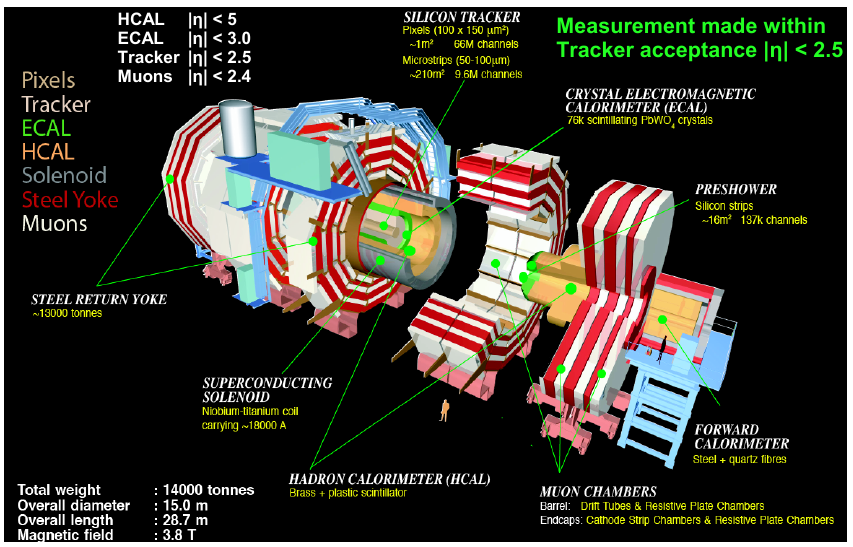
\includegraphics[scale=0.6]{THESISPLOTS/CMS-Detector.png}} 
\captionof{figure}{CMS Detector with colors indicating different subdetectors.}
\label{fig:CMS-DET}
\end{center}
The CMS detector performance can be summarised as seen in table \eqref{CMSRES} with the material type in each sub-detector.

\begin{center}\label{CMSRES}
\begin{minipage}[b]{1.0\linewidth}
\centering
 %\setlength{\abovecaptionskip}{0pt}
  %\setlength{\belowcaptionskip}{10pt}
 % \topcaption{GMSB,GGM Phenomenology and Relevant final states}
  \begin{tabular}{|l|l|p{3.2cm}|p{3.9cm}|}
  \hline \hline
  \multicolumn{4}{|c|}{\bfseries{CMS Detector and Resolution}} \\
  \hline \hline
  \bfseries{Subdetector} & \bfseries{Quantity} & \bfseries{Resolution} & \bfseries{Uses}  \\
   \hline \hline
 Tracker   & Momentum[GeV/c]  & $\sigma_{T}/p_{T} \approx 1.5\times 10^{-4}p_{T} + 0.005$ & \mbox{Silicon Pixels and Strips} \\ 
  \hline
  ECAL   & Energy[GeV] & $\sigma/E \approx 3\% /E + 0.003$ & $\pb$ Crystals \\
   ECAL  & Time[ns] & $\sigma(\Delta t)= \frac{N}{A_{eff}/\sigma_{n}}\oplus\sqrt{2}\bar{C} $ & $\pb$ Crystals \\
  \hline
  HCAL & Energy[GeV] & $\sigma/E \approx 100\% /E + 0.05$ & Brass + Scintilator\\
  \hline
  Muon Chambers & Momentum[GeV/c] & $\sigma_{T}/p_{T} \approx$ 1\%  \@ 50 GeV to  10\% \@ 1 \TeV & inner tracker + Muon Systems \\
  \hline
  Magnetic field & B-field strength[T] & 3.8~T + 2~T & Solenoid + Return Yoke\\
  \hline
  Triggers  & On/Off-line & Levels &\mbox{L1(On-line)} +\mbox{HLT(Off-line)}(L2+L3) \\
  \hline
  \hline
  \end{tabular}
  \captionof{figure}{CMS Detector Material and Resolution(Time resolution: $N\approx 35$~ns, $\bar{C}\approx 0.020$~ns \cite{Time})}
 \end{minipage}
 \end{center}

The coordinate system used by the CMS  is such that the origin is centered at the nominal collision point inside the detector. The direction of $x,y,$ and $z$-axis pointing towards the Jura Mountains from P5 are shown in figure \eqref{CMSCORD}. However, the CMS often uses the azimuthal angle $phi$ measured from the $x$-axis in the $x-y$ plane and the radial distance in this plane. The polar angle $theta$  measured from the $z$-axis is related to the \textit{pseudo-rapidity}, $\eta$ through the relation: $$\displaystyle{\eta = -\ln \tan(\frac{\theta} {2}) } $$. The co-ordinate system $(\eta, \phi, z)$ and its radial distance $r$ defines a point in the CMS detector whose volume is a cylinder. 
\begin{center}\label{CMSCORD}
\centering
\mbox{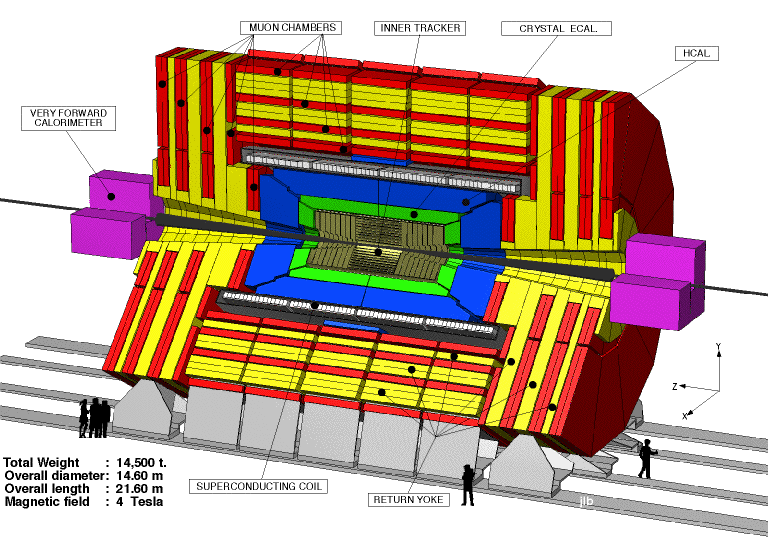
\includegraphics[scale=0.4]{THESISPLOTS/cms-Dect-Cord.png}} 
\captionof{figure}{Schematic diagram of CMS detector view showing definition of cordinates as used by CMS.}
\label{fig:CMS detector showing defination of coordinates.}
\end{center}

CMS defines quantities such as \textit{transverse momentum}~($p_{T}$), \textit{transverse energy}~($E_{T}$) and \textit{transverse missing energy}~($\MET$ or MET ) to distinguish quantities in the transverse plane($x-y$ coordinate) from those along the longitudinal direction($z$ coordinate) or beam line. It also uses a cone-like structure where the cone radius is defined as $$\displaystyle{ \Delta R = \sqrt{ \Delta\eta^{2} + \Delta\phi^{2} } }$$ to measure the distance between two objects in the $\eta-\phi$ plane. Cone-like structures are used for particle isolation and identification purposes.


\subsection{Tracker}




\subsubsection{Pixel}
\subsubsection{Silicon Strip Tracker}
Unlike calorimeters, the tracker is basically a magnetic spectrometer where the momentum resolution is linearly  proportional to the particle's momentum 
 in a given  magnetic field.
 This means very low momentum particles have better momentum resolution than their high momentum counterparts.
 The momentum of a charged particle is inversely proportional to the curvature of its trajectory in the magnetic field. 
 By reconstructing the trajectory of the particle as it moves in the tracker; through ``hits'' made at various positions,
 we are able to deduce its curvature and hence determine its momentum.
 High momentum particles are less curved by the magnetic field than low momentum particles.
Thus, the tracker  is expected to have a very good momentum resolution for low momentum particles. The strong magnetic field and high granularity of the 
CMS silicon tracker allows promptly produced charged particles with $\PT = 100GeV/c$ to be reconstructed with a resolution in the transverse momentum \PT  of
 about $\sim 1.5\,\%$.
 The tracker and calorimeter combine to provide good energy resolutioin for low as well as high momentum particles respectively.
\paragraph*{} 
At the LHC design luminocity of $10^{34}~cm^{-2}s^{-1}$ there will be on average $1000$ particles from roughly $23$ overlapping proton-proton interactions traversing
the tracker for each bunch crossing every $25$~ns. A detector technology featuring high granularity and fast response is required such that the trajectories can be identified
reliably and attributed  to the correct bunch crossing.
It is for this reason that the CMS tracker opted for silicon technology. Since silicon sensors are highly suited to receive many particles in a small space 
due to  their fast response  and spatial resolution.
The tracker is tasked along with the ECAL and  muon chambers to identify electrons and muons. Tracking information is also heavily used in the High Level
Trigger (HLT) system of the CMS to reduce the event rate from the LHC bunch crossing rate of $40~MHz$ to about $100~Hz$ which can be permanently stored.
One of the most important goals of the tracker is to minimize the effects on the tracking performance of electron bremsstrahlung and hadronic interactions. For this,
the tracker has a track isolation criteria for identifying photons and electrons from electromagnetic clusters. This criteria is applied to suppress
$\gamma-\pi^{o}(jet)$ and $\pi^{o}-\pi^{o}(jet-jet)$ backgrounds to a level significantly below the irriducible $\gamma-\gamma $ background.
\newline
The CMS tracker achieves this performance by using silicon pixel and  strip trackers. It has about 1440 pixel and 15148 strip detector modules.
The pixel tracker has 3 layers positioned at
radii between 4.4~cm and 10.2~cm while the silicon strip tracker has 10 layers surrounding the pixel detector in the barrel and extending out ward to  a radius of 1.1~m.
Each system is completed by endcaps which consist of 2 disks in the pixel detector and 3 plus 9 disks in the  strip tracker on each side of the barrel extending
the acceptance of the tracker to a pseudorapidity of $\vert\eta\vert < 2.5$. The pixel detector also covers a pseudorapidity  of $ -2.5 < \eta < 2.5$ matching the acceptance of the
 central tracker. It is closest to the beam line directly surrounding the interaction vertex and has
pixels of size $\approx 100 \times 150~\mu m^{2}$ covering a total area of $\approx 1~m^{2}$. The main function of the pixel detector is to provide  precise tracking points
in the $ r-\phi$ and Z responsible for small impact parameter resolution of about $\sim 15~\mu m$  ~\cite{CMSTDR},which is important for
good secondary vertex  reconstruction and position resolution. This is crucial in the identification of  displaced vertex physics objects with life-time of 
about $\tau \approx 10^{-12}~s$. They include particles such as
$B^{0,{\pm}}$, $D^{0,{\pm}}$, $\tau^{\pm}$, which may travel a distinguishable distance (c$\tau$ $\approx 100~\mu$m.) 
before decaying into particles with tracks like electrons and muons. 
In addition, it is also important for forming seed tracks for outer track reconstruction and high level triggering.
\newline
 %The tracker consists of the Silicon Strip Tracker(SST) and Pixel Tracker.
 %Its volume consists of a first layer of pixels followed by strips extending to ~$110$~cm with a total length of 540~cm. 
 %Ecah pixel has a size $\approx 100 \times 150~\mu m^{2}$ providing good vertex and position resolution.
 %Close to the interaction vertex, in the barrel region are 3 layers of hybrid pixel detectors at a radii 4.4, 7.3, and 10.2~cm.
 The silicon strip detector covers the radii region $ 20$~cm$ < r < 110$~cm.
 The over 15,000 silicon modules occupy an active area of $200~m^{2}$ providing a coverage in pseudorapidity up to
 $\vert\eta\vert < 2.5 $. It is also known as the outer tracker and consist of almost 9.6 million silicon strips providing a 
 spatial resolution measured to be about $10~\mu$m for $r-\phi$ measurement and about
$20~\mu$m for Z measurment necessary for particle trajectory reconstruction.
At the intermediate radii ($ 20$~cm$ < r < 55$~cm), where the particle flux is reduced, it is instrumented with silicon micro strip in the barrel detector
with a typical cell size of
$10~cm \times 80~cm$ in $ r-\phi $ and Z plane. The silicon modules here have sensors of thickness about $320~\mu m$,
while for radial distances; $ 55$~cm$ < r < 110$~cm, the strip detector uses longer strips. The strip electric noise scales linearly with its length. Thus in order
to maintain a good signal to noise ratio well above 10, the CMS uses thicker silicon sensors of about $500~\mu m$ which has correspondingly higher signal.
Overal the Strip detector is made of 4 subdetectors. The Inner Barrel (TIB) consists of 4 cylindrical layers while the outer barrel (TOB) has 6 cylindrical layers.
Two endcap detectors(TEC) in the positive and negative side of the Z cordinate consist of 9 carbon fiber disks with petal structure providing support for the modules.
Signals from  modules of both strip and pixel dectors are amplified by 4 to 6 Analogue Pipeline Voltage(APV25) read out chips mounted on the front-end hybrid(FE-hybrid).
The hybrid provide key information such as temperature of the chips and timing information in order to match the recorded ``hits'' with collision.
 
%Measuring the track of charge particles in the tracker provide enough information to calculate it's momentum.
%The inner tracker measures charged particles within the $\vert\eta\vert < 2.4$ pseudo-rapidity range.% It is located in the 3.8T field of the superconducting solenoid. 
%It provides and impact parameter resolution of $\sim 15~\mu m$ and a $\PT$ resolutions of about $1.5\,\% $ for 100~GeV/c particles ~\cite{CMSTDR}
%\newline
% A detailed description of CMS  detector can be found elsewhere ~\cite{JINST}.
\subsection{Calorimeter}
Calorimeters have a unique property of improving relative energy resolution with increasing energy thus making them indispencable  in high energy physics experiments.
In the decay of neutralino, we espect the photon produced to have a very high energy(above 90GeV) and the gravitino which is weakly interacting to emerge as large missing energy.
Therefore it is imperative to describe how the calorimetry system of CMS is designed to ensure that we can detect these photons. We also provide a brief description of
 the tracking system use for calculating missing transverse energy
\subsubsection{Electromagnetic Calorimeter}
 The Ecal consists of the Barrel(\textsc{EB}) region occupying a pseudo-rapidity of $\vert \eta \vert< 1.479 $ and two Endcaps (\textsc{EE}) regions covering $1.479 <\vert \eta \vert < 3.0$.
 Sitting right in front of the \textsc{EE}, is a Preshower(\textsc{ES}) detector made of silicon strip sensors interleaved by lead making it a few radiation length thick.
 Its main purpose is to improve in $\gamma/\pi^{0}$ descrimination in the \textsc{EE} regions.
 \paragraph*{}
 The \textsc{EB} and \textsc{EE} combined consist of 75848 lead tungstate (\pb) scintinlating crystals. At the longitudinal end of each crystal is coupled two 
 Avalanche-Photodiodes(APDs) for \textsc{EB} crystals and  Vacuum-Phototriodes(VPTs) for \textsc{EE} crystals for scintilating light collection developed in the crystals.
 VPTs are used for \textsc{EE} crystals because of their better resistance against high radiation.
 This large number of crystals provide an almost $4\pi$ coverage of solid angle which is important for missing energy calculation. 
 \newline 
 \pb  has a radiation length ($X_{0}$) of $\simeq 0.89$~cm. The total longitudinal length of a crystal in  \textsc{EB} is $ 25.8X_{0}$ and $24.7X_{0}$ in \textsc{EE}
 providing enough absorber thickness for most of the energy of the incident very energetic photon or electron to completely lose through a 
 cascade process in the crystal. This energy loss is mainly through radiation of photons(\emph{Bremsstrahlung}) and pair production. The ``amplitude'' or ``probability'' of these processes is 
 proportional to the nuclear charge or number of electrons, \text{Z} of the material. \pb is a high \text{Z} material which makes it a good choice along
 with other properties like fast scintilation time for ECAL calorimetry. Low energy electrons lose their energy through other processes like ionization and excitation. 
 Eventhough \pb is a heavy material, Compton scattering and photoelectric effect is still possible as most of the photons with energy below a few \MeV have 
 their dominant contribution to energy loss from mainly  these processes.
 \newline
 \pb crystals also have a Moliere radius of $2.4$~cm. This ensures that on average about $95$\,\% of the electromagnetic shower energy is contained within the crystal volume therefore
 reducing the transverse spread of the electromagnetic cascade arising from multiple scattering of electrons. It improves on the estimation of the transverse position
 of impact of the incident particle. This  Moliere radius implies \pb is very dense and compact therefore resistant 
 to radiation making it suitable for a high radiation environment like the LHC.
 \newline
 The crystals are  tapered and arranged in a projective goometry pointing $\approx3^{o}$ away from the mean beam collision point. The purpose
 of this is to minimize inter crystal gaps hence preventing photons or part of the photon cluster from going through these gaps undetected.
 This improves the energy calibration and reduces the contribution to the constant term in the Ecal energy resolution and is the dominant
 contribution for high energies and in missing energy calculations. 
 \newline 
 \pb has a fast( 80\,\% of the light emitted within $25$~ns) scintilation process. It peaks in the blue region ($425$~nm) making photo-detection simpler and reliable in a fast
 (bunch crossing frequency of $40$~MHz) timing requirement environment like the LHC.
Although the light-yield for \pb is rather low ($\approx 70$photons/\MeV), the photodiodes have internal gain ( $50$ for APDs and 10 for VPTs) and good quantum efficiency
of $75$\,\% for APDs and $20$\,\% for VPTs of the emission wavelength. This makes it possible that signals 
from incident particles with energies from a few  to high \GeV can be recorded.
\paragraph*{}
 This homogenous design of the ECAL provides it with a performance which is optimal(by design) in its potential to discover a Higgs in the mass region 
 less than $130$\GeV/$c^{2}$ through the decay $\displaystyle{H\rightarrow\gamma\gamma}$. 
 Homogenous design implies reduced noise in the detector  thus better resolution since only a single material type is in use.
ECAL has a current  timing resolution better than 500~ps for large energy deposits(more than 10-20~GeV in the \text{EB})~\cite{TIME} 
and an energy resolution of ${\displaystyle\sigma/E\approx 0.45\,\%}$ for unconverted photons with energies above 100~GeV~\cite{CMSTDR}.
 
% \subsubsection*{The Readout Chain}
%The scintillation time (~25~ns), small radiation length (9 mm), and radiation hardness of PbWO$_4$ are the reasons 
%that this material was chosen for CMS since they minimize the overlapping of signals in space as well as interactions in the 
%adjacent bunch crossings, and they survive in a high radiation environment of the LHC.
%ECAL consists of $75848$ lead tungstate (\pb) scintilating crystals providing a coverage in pseudo-rapidity  of $\vert \eta \vert< 1.479 $ in a barrel
%region (\textsc{EB}) and $1.479 <\vert \eta \vert < 3.0$ in two endcap regions (\textsc{EE}) to cover a large solid angle region, which is important for minimising 
%false missing transverse energy.
%Because of the relatively fast scintillation decay time, we are able to measure the time of the signal very well, and we take advantage of this for our analysis of delayed photon.
%The timing resolution of ECAL Crystals is better than 500~ps for large energy deposits(more than 10-20~GeV in the barrel)~\cite{TIME}.
 %In fact, \pb has a decay time of 25~ns which is comparable with the LHC bunch  crossing interval of 25~ns.
%This extremely fast scintillation process makes it an excellent material in an environment like the LHC.
% \newline
%The signal is generated in the \pb crystals through an electromagnetic showering process.
%This process is caused by electromagnetic interactions between  high energy photons and electrons through a process called
%\emph{Bremsstrahlung} and pair-production. During pair production, the incoming photon, interacts with the atom to produce an electron and positron pair.
%However, in bremsstrahlung, the energetic electron interacts with the nucleus of the atom and is then accelerated
%such that the accelerated electron radiates off a photon continuing as a less
%energetic  electron. The emitted photon can later pair-produce.
%The continuous Bremsstrahlung and pair-production leads to a cascade  production of photons and electrons called the electromagnetic shower.
%It eventually stops when the photons or electrons become less energetic enough to either pair-produce or bremsstrahlung.
%The light produced by the crystals is collected by photo devices which converts this light into photo current and is then transmitted
%eventually to the front end detector. %After every 25ns, through high-speed data link per crystal, all data is  transported out of the ECAL into the counting room.
%\newline
%In front of the \textsc{EE},
%is a single radiation length thick lead material called, the preshower detector. It consist of two planes of silicon sensors interleaved
%with a 9~mm thickness of lead. Its main purpose is to provide $\pi^{0}-\gamma$ separation by distinguishing converted from unconverted photons.%

 %A  unique capability of crystal total absorption calorimetry is its excellent energy resolution. % and hermetic coverage.
%The CMS ECAL utilizes lead tungstate (PbWO$_4$) crystals to achieve an energy resolution of ${\displaystyle\sigma/E\approx 0.45\,\%}$ 
%for unconverted photons with transverse energies above 100~GeV~\cite{CMSTDR}.
% 
% \subsubsection{ECAL}
%  A  unique capability of crystal calorimetry is its excellent energy resolution and hermetic coverage.
% The CMS ECAL has  an energy resolution of ${\displaystyle\sigma/E(GeV)\approx 0.45\,\%}$.
% It consist of nearly $75848$ lead tungstate (\pb) scintilating crystals providing a coverage in pseudo-rapidity  of $\vert \eta \vert< 1.479 $ in a barrel
% region (\textsc{EB}) and $1.479 <\vert \eta \vert < 3.0$ in two endcap regions (\textsc{EE}).
%  %The lead-tungstate crystals provides a fine granularity of $\Delta\eta\times\Delta\phi=0.0175 \times\ 0.0175$ and $\Delta\eta\times\Delta\phi=0.0175 \times\ 0.0175$ to 
% %$\Delta\eta\times\Delta\phi=0.05 \times\ 0.05$ for \textsc{EB} and \textsc{EE} respectively. 
% It  has a radiation length of $X_0=0.89$cm. This allows for much of the energy lost through radiation before eventual ionization.
% The crystals are arranged with a longitudinal length of 25.8\,$X_0$ in the barrel and 24.7\,$X_0$ in the endcaps, 
% such that the scintilation light produced from each crystal is finely collected by photodiodes glued at the end of each crystal.
% Avalanche Photodiodes(APDs) is used for \textsc{EB} and  Vacuum Phototriodes(VPTs) for \textsc{EE}. These photodiodes have high gain and are less affected by
% the high magnetic field. 
% Energy from incoming particles is converted into light through a process called scintillation. 
% The \pb have a unique property in that, in about 25ns, about 80\,\% of all the incomming particle's energy  used to excite the atoms, is released through the scintillation process.
%  In fact, \pb has a decay time of25ns which is comparable with the LHC bunch  crossing interval of 25ns.
% This extremely fast scintillation process makes it an excellent scintilating  material in a fast decision making and high luminosity region like the LHC.
% The electromagnetic showering process is caused by electromagnetic interactions between  high energy photons and elections through a process called
% \emph{Bremsstrahlung} and pair-production. During pair production, the incoming photon, interacts with the atom to produce an electron and positron pair. 
% Where as, in bremsstrahlung, the energetic electron interacts with the nucleus of the atom and is then accelerated 
% such that the accelerated electron radiates off a photon continuing as a less
% energetic  electron. The emitted photon can later pair-produce. 
% The continuous Bremsstrahlung and pair-production leads to a cascade  production of photons and electrons called the electromagnetic shower.
% The process eventually ends when the photons or electrons become less energetic enough to either pair-produce or bremsstrahlung.
% The scintiallated light is collected by the APDs and VPTs which converts this light into photo current and is then transmitted 
% eventually to the front end detector. After every 25ns, through high-speed data link per crystal, all data is  transported out of the ECAL into the counting room.
% \newline
% In front of the \textsc{EE}, 
% is a single radiation length thick lead material called, the preshower detector. It consist of two planes of silicon sensors interleaved 
% with a total of 3$\,X_0$ of lead. Its main purpose is to provide $\pi^{0}-\gamma$ separation by distinguishing converted from unconverted photons.
\subsubsection{Hadronic Calorimeter}
The forward hadronic calorimeters placed upstream have scintillating tiles called Beam Scintillation Counters~(BSC) which in coincidence with beam pick-up monitors ~(BPTX) helps to eliminate beam background contamination at the trigger level.
Directly behind the ECAL, is the hadronic calorimeter(HCAL).
Unlike the homogeneous ECAL, the HCAL is an inhomogeneous sampling calorimeter. 
The  hadronic barrel(\text{HB}) and hadronic endcap(\text{HE}) of the HCAL cover a region in pseudo-rapidity of $\vert \eta \vert < 3$. 
The designed consist of plastic scintilating tiles with wavelength shifting fibers sandwiched between layers of brass or steel as absorber giving 
it a repeated interleaved structure  of absorber/dead( steel or brass)  
and active layers of tiles of  plastic scintilating material. The active material
is used mainly for periodically sampling electromagnetic and hadronic components in the hadronic shower 
while steel and brass act as stopping material for energetic incoming hadrons in the shower.
The  absorber material provide fine granularity  of short  nuclear interaction length while tiles of plastic scintilator
separates charged hadrons like protons, pions($\pi^{\pm}$), kaons($k^{\pm}$)  and neutrons from
electromagnetic physics objects like photon and neutral pions contained in the incident hadronic shower. 
This ability to separate different components of a hadronic shower serves as the basis for some particle reconstruction algorithms making the HCAL 
very usefull in the reconstruction of complex physics objects 
like jets which usually consist of hadronic as well as electromagnetic showers.
The HCAL is thus very important in missing energy calculation.
Quartz fibers for Cerenkov light production placed in a steal mix occupy $3 < \vert \eta \vert < 5$.
 % like Particle Flow analysis(\text{PF}).
 \newline
This inhomogenous design gives the HCAL, an energy resolution of ${\displaystyle \Delta E/E \approx 0.5/\sqrt{E(GeV)} }$ above 250~GeV ~\cite{CMSTDR}.
\paragraph*{}
The HCAL calorimeter  is a sampling calorimeter which means it finds the particle's position, energy and arrival time by using the alternating layers of ``absorber''
and fluorescent ``scintilating'' materials which produce a rapid light pulse when  a particle passes through. Some special optic fibres  collect up this light and supply it
to readout boxes where photodetectors amplify the signal. The amount of light in a given region is summed up over many layers of tile along the 
particle's path through the HCAL in depth called a ``tower''. The total amount of light is a measure of the particle's energy and an indicator of its type.
This sampling is used to separate the hadronic  and energetic  electromagnetic  component of the shower which passed through the ECAL unstopped.
\newline
A hadronic shower is formed when an incident hadron undergoes an inelastic collision with the nucleus of the absorber material 
producing secondary hadrons which as they go through successive layers of
absorber material interact inelastically with other nuclei to produce further hadrons etc. 
The  hadronic cascade loses about 30\,\% of incident hadron energy through nuclear excitation of the nuclei of atoms of the  absorber material.
\newline
The HB calorimeter is an assembly of two half barrels each composed of 18 identical
$20^{o}$ wedges in $\phi$. The wedge is made of flat brass alloy absorber plate parallel to beam axis with the innermost and outermost layers made up of
stainless steal interleaved by plastic scintillating tiles.
The first active layer is situated directly behind the ECAL in order to actively sample low energy showering particles from the support material between the ECAL 
and HCAL. Each scintillating tile has a size of $\Delta\eta\times\Delta\phi=0.087 \times\ 0.087$ 
and is instrumented with a single wave length shifting fiber(WLS) for better collection of light. The summed optical signals or light are converted into fast electronic
signals by photo-sensors called  hybrid photo-diode(HPD).
%The optical signal from the HCAL towers is detected with a pixelated
\newline
In the forward region in $\eta$ is the forward calorimeter (HF) made up of steel absorbers embedded in radiation hard quartz fibers running parallel to the 
beam axis and providing a fast collection of Cherenkov light. The signal results from Cherenkov light emitted in the quartz 
fibres embedded in the steel matrix in response to charged particles.
The Cherenkov calorimeter have long and short fibers which are positioned alternatively separated by 5~mm with readouts for better 
sampling of the different shower components.
The goal of this hardware design is to give better compensation for different shower components in the hadronic shower.
The HF section enables the HCAL to pick up myriad of particles coming out of the collision region  at very shallow angles relative to the beam direction.
%In fact the steel and brass alloy sandwiched with active tile of scintillator provide a great stopping power for highly energetic events as well as providing fast readout.
\newline
These different sections of the HCAL in $\eta-\phi$ plane give it a unique capability to measure multi-jet events revealing the fine structure of jets.
Decaying particles may produced new particles that do not leave any record  of their presence in any part of the CMS detector.
To spot such particles, the above HCAL sections give it an almost ``hemetic'' coverage making sure it captures  to the extend possible every particle emerging from
collisions.  In this way, if we observe a particle in one side of the detector but not in the other, with imbalance of momentum and energy in the direction
``transverse'' to the beam  direction, we can deduce that we are producing ``invincible''     particles. 
This is the primary idea in missing transverse energy calculation  established as signal for very weakly interacting particles like neutrino and hopefully gravitino.
Generally speaking, in the region $\vert \eta \vert< 1.74$, the HCAL cells have widths of 0.087 in pseudorapidity($\eta$) and 0.087\,rad in azimuth ($\phi$).
In the $(\eta,\phi)$ plane, and for $\vert \eta \vert < 1.48$, 
the HCAL cells map on to $5 \times 5$ ECAL crystals arrays to form calorimeter towers projecting radially outwards from close 
to the nominal interaction point. At larger values of $\vert \eta \vert$, the size of the towers increases and the matching ECAL arrays contain fewer crystals. 
Within each tower, the energy deposits in ECAL and HCAL cells are summed to define the calorimeter tower energies subsequently used to provide the energy
 and direction of hadronic jets. 
% \newline
% All these information is fed into the PF algorithm for particle reconstruction.
\subsection{Muon Chambers}

%%%%%%%%%%%%%%%%%%%%%%%%%%%%%%%%%%%%%%%%%%%%%%%%%%%%%%%%%%%%%%%%%%%%%
A complete picture showing CMS sub-detectors definitions in terms of coordinates can be seen in figure \eqref{CMS-SUBD}
\begin{center}\label{CMS-SUBD}
\centering
\mbox{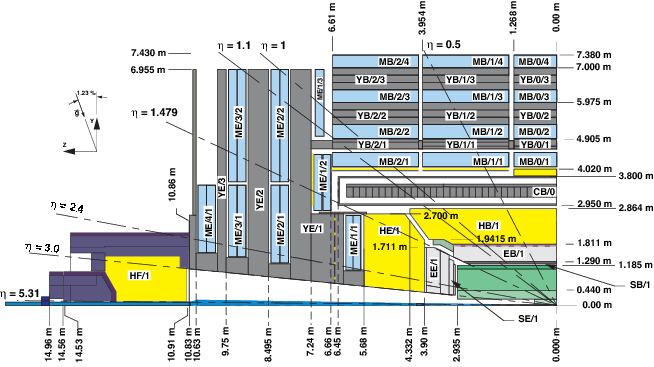
\includegraphics[scale=0.6]{THESISPLOTS/CMS_Int_View.png}} 
\captionof{figure}{Longitudinal view of CMS showing the coverage range of its sub-detectors.}
\label{fig:CMS Detector Longitudinal view.}
\end{center}



\subsection{Particle Detection}
Using the above CMS sub-detectors, particle detection is done using information from every sub-detector.
The figure \eqref{CMSSLICE} show a  transverse slice of the CMS detectors with tracks and energy deposit showing how different particles interact with the material in different sub-detectors thus ensuring their unique identification and reconstruction in the detector.
 
\begin{center}\label{CMSSLICE}
\centering
\mbox{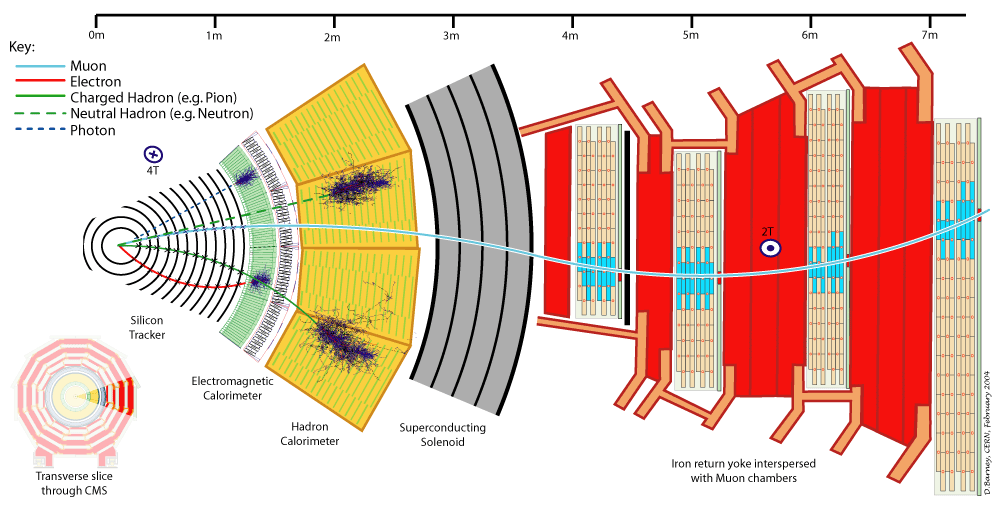
\includegraphics[scale=0.4]{THESISPLOTS/CMS_Slice.png}} 
\captionof{figure}{Transverse slice of the CMS detector showing how different types of particles interact and hence identified using this detector.}
\label{fig:CMS SLICE}
\end{center}

\label{Collider_And_Detector_chapter}
%%%%%%%%%%%%%%%%%%%%%%%%%%%%%%%%%%%%%%%%%%%%%%%%%%%%%%%%%%%%%%%%%%%%%%%%%%%%%%%%
